\chapter{Implementation Overview}

\section {Idea behind the project} 
As already stated, the goal of this project is to provide a secure PUF to check the authenticity of IoT devices in order to avoid impersonation attacks. The proposed solution shows how an SRAM PUF can be implemented. The used SRAM is part of a SECube\textsuperscript{TM} device.

The main idea behind this implementation of an SRAM PUF is that whenever the host tries to connect with the SECube\textsuperscript{TM}, a challenge-response mechanism will take place in order to establish that the SECube\textsuperscript{TM} the host wants to connect to, is the original one and that it has not been replaced. 
The first time the host connects with the SECube\textsuperscript{TM}, it asks the device to send back a list of strings (which will be called \emph{responses}). These strings are the initial values that the SRAM assumes before being overwritten. At power on, each SRAM cell always tends to have the same stable state (a \emph{0} or a \emph{1}), i.e., each cell always assumes the same state every time it is powered on. The values of this cells cannot be predicted or simulated since they depend on the physical implementation of the SRAM (see \ref{section:physicalUnclonableFunctions} for more details). 
The first time the host receives these responses from the device it wants to connect to, it stores them in a file that will be used as a database to be used for future authentication checks.

In later connections with the device, the host sends a challenge to the device it wants to connect to and waits for a response. This challenge is the address location whose content will be checked by the host against the dabase of values it has previously stored during the first connection with the device. When the device receives the challenge, it reads the content of the address and sends a response back to the host. The host then checks if the response it has received matches with the one stored in the database and it can therefore asssess if the device it is trying to connect to is the real one.

%\begin{equation}\label{eq:eq1}
% data\_to\_store=H(response)
 %\end{equation}

%In the future when the host has to establish a connection with the device, he is going to send to it a specific challenge, the device is going to answer with a response;
%then the host has to check the validity of the response, evaluating the digest and comparing with the one that he has in the storage file.


\section{Implementation overview}
The implementation of this project can be divided into two flows:
\begin{enumerate}
	\item The first flow consists in the host retrieving all the responses from the device 
	\item The second flow consists in the challenge-response authentication mechanism between the host and the device 
\end{enumerate}

\begin{figure}[H]
\centering
  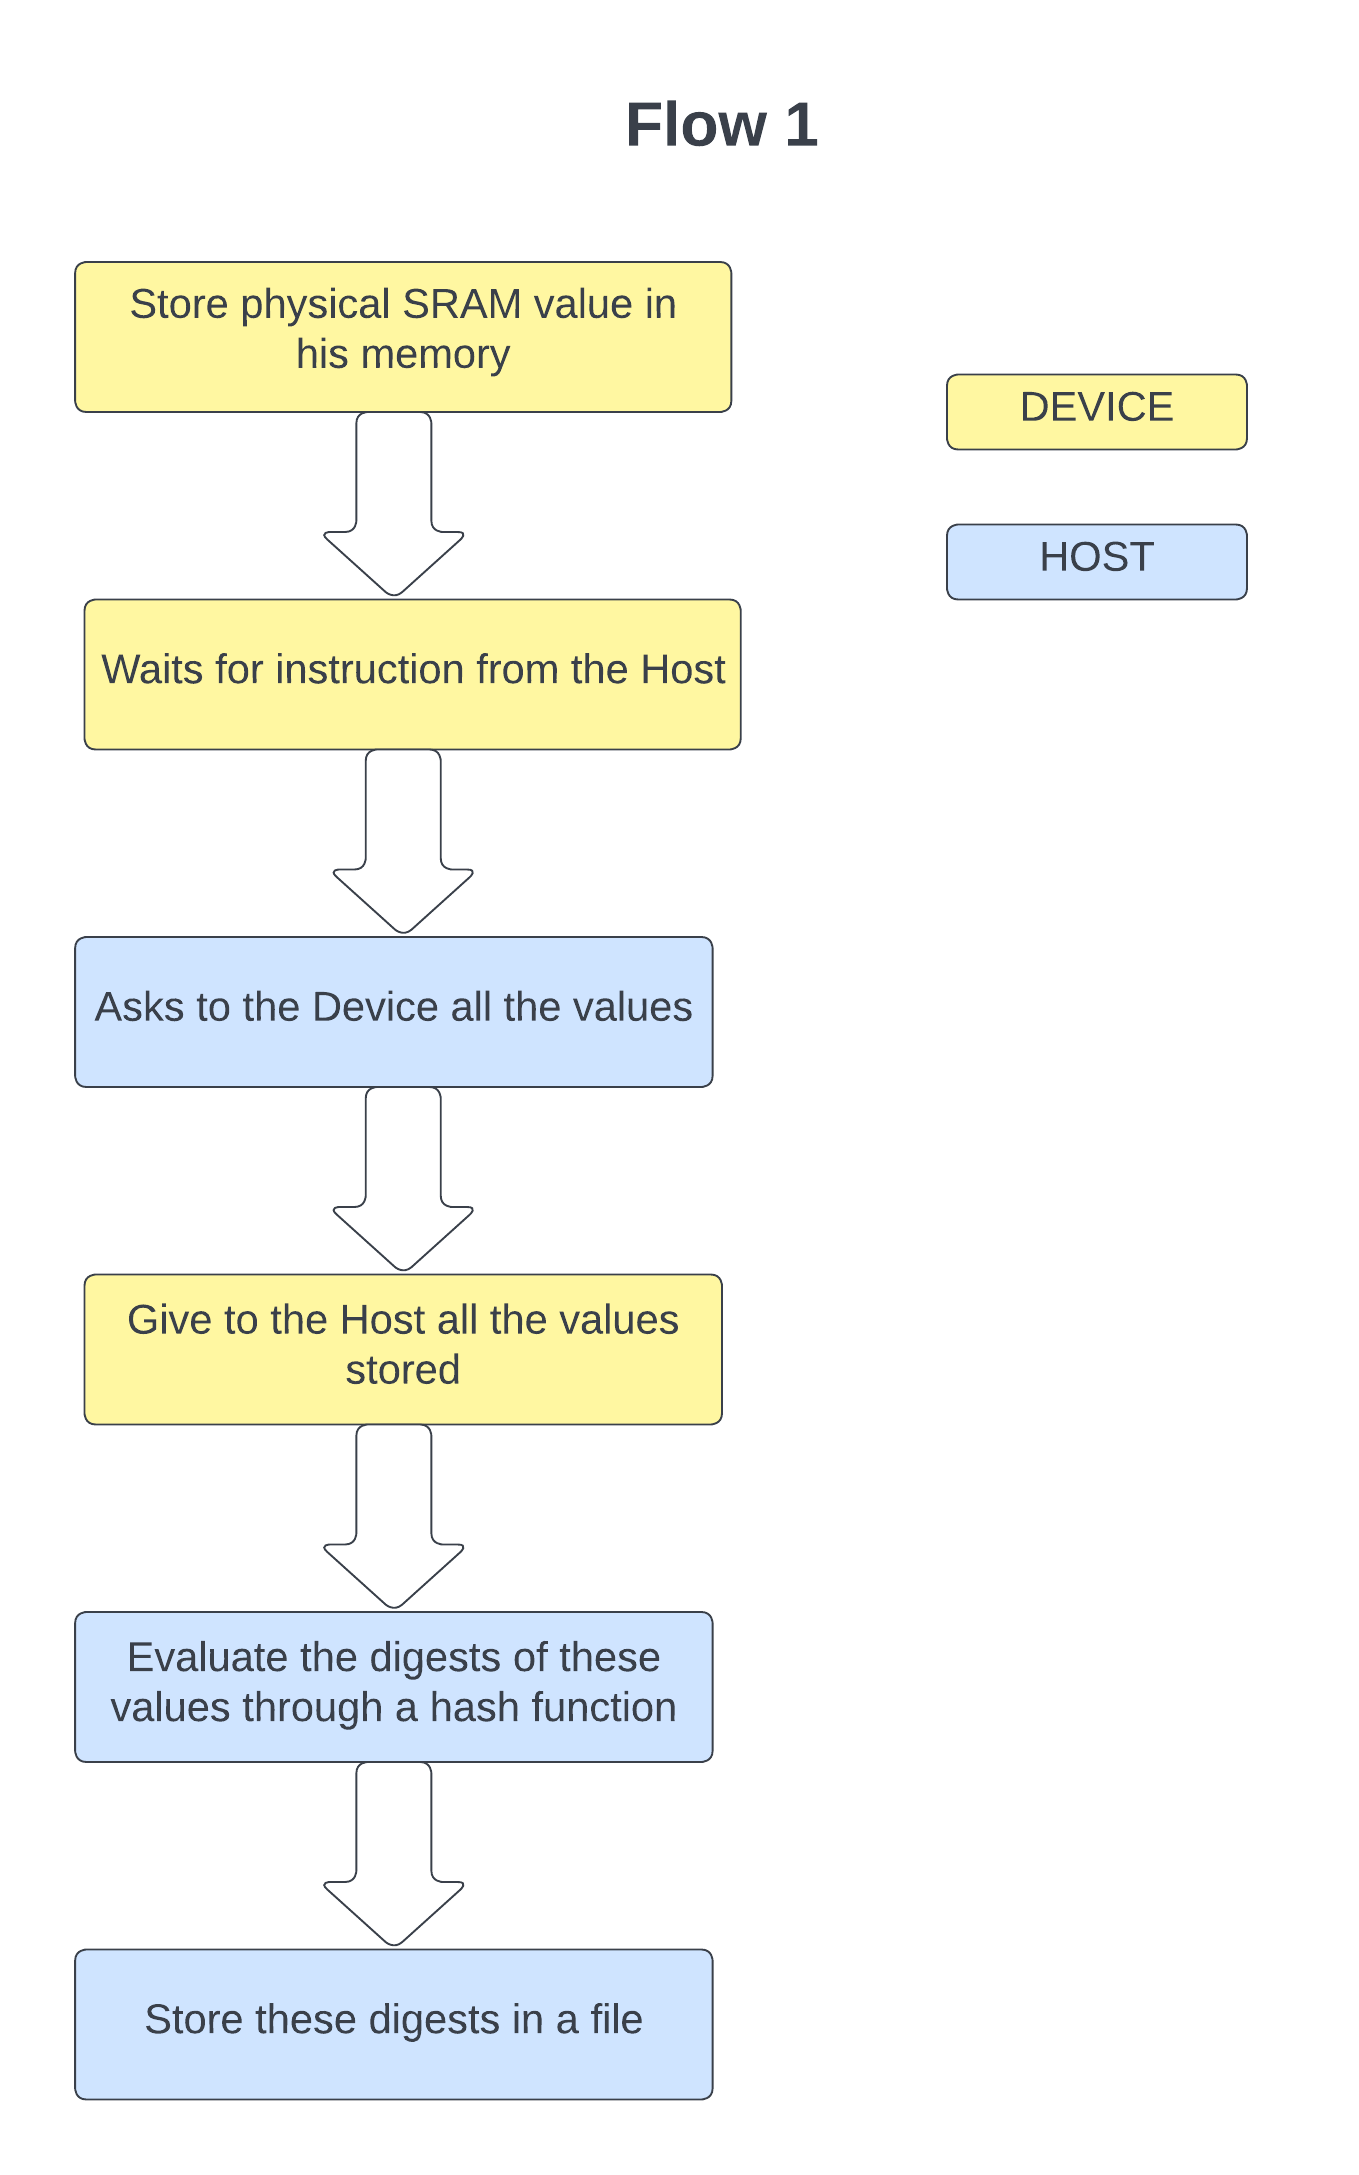
\includegraphics[width=5cm]{images/flow_1.png}
  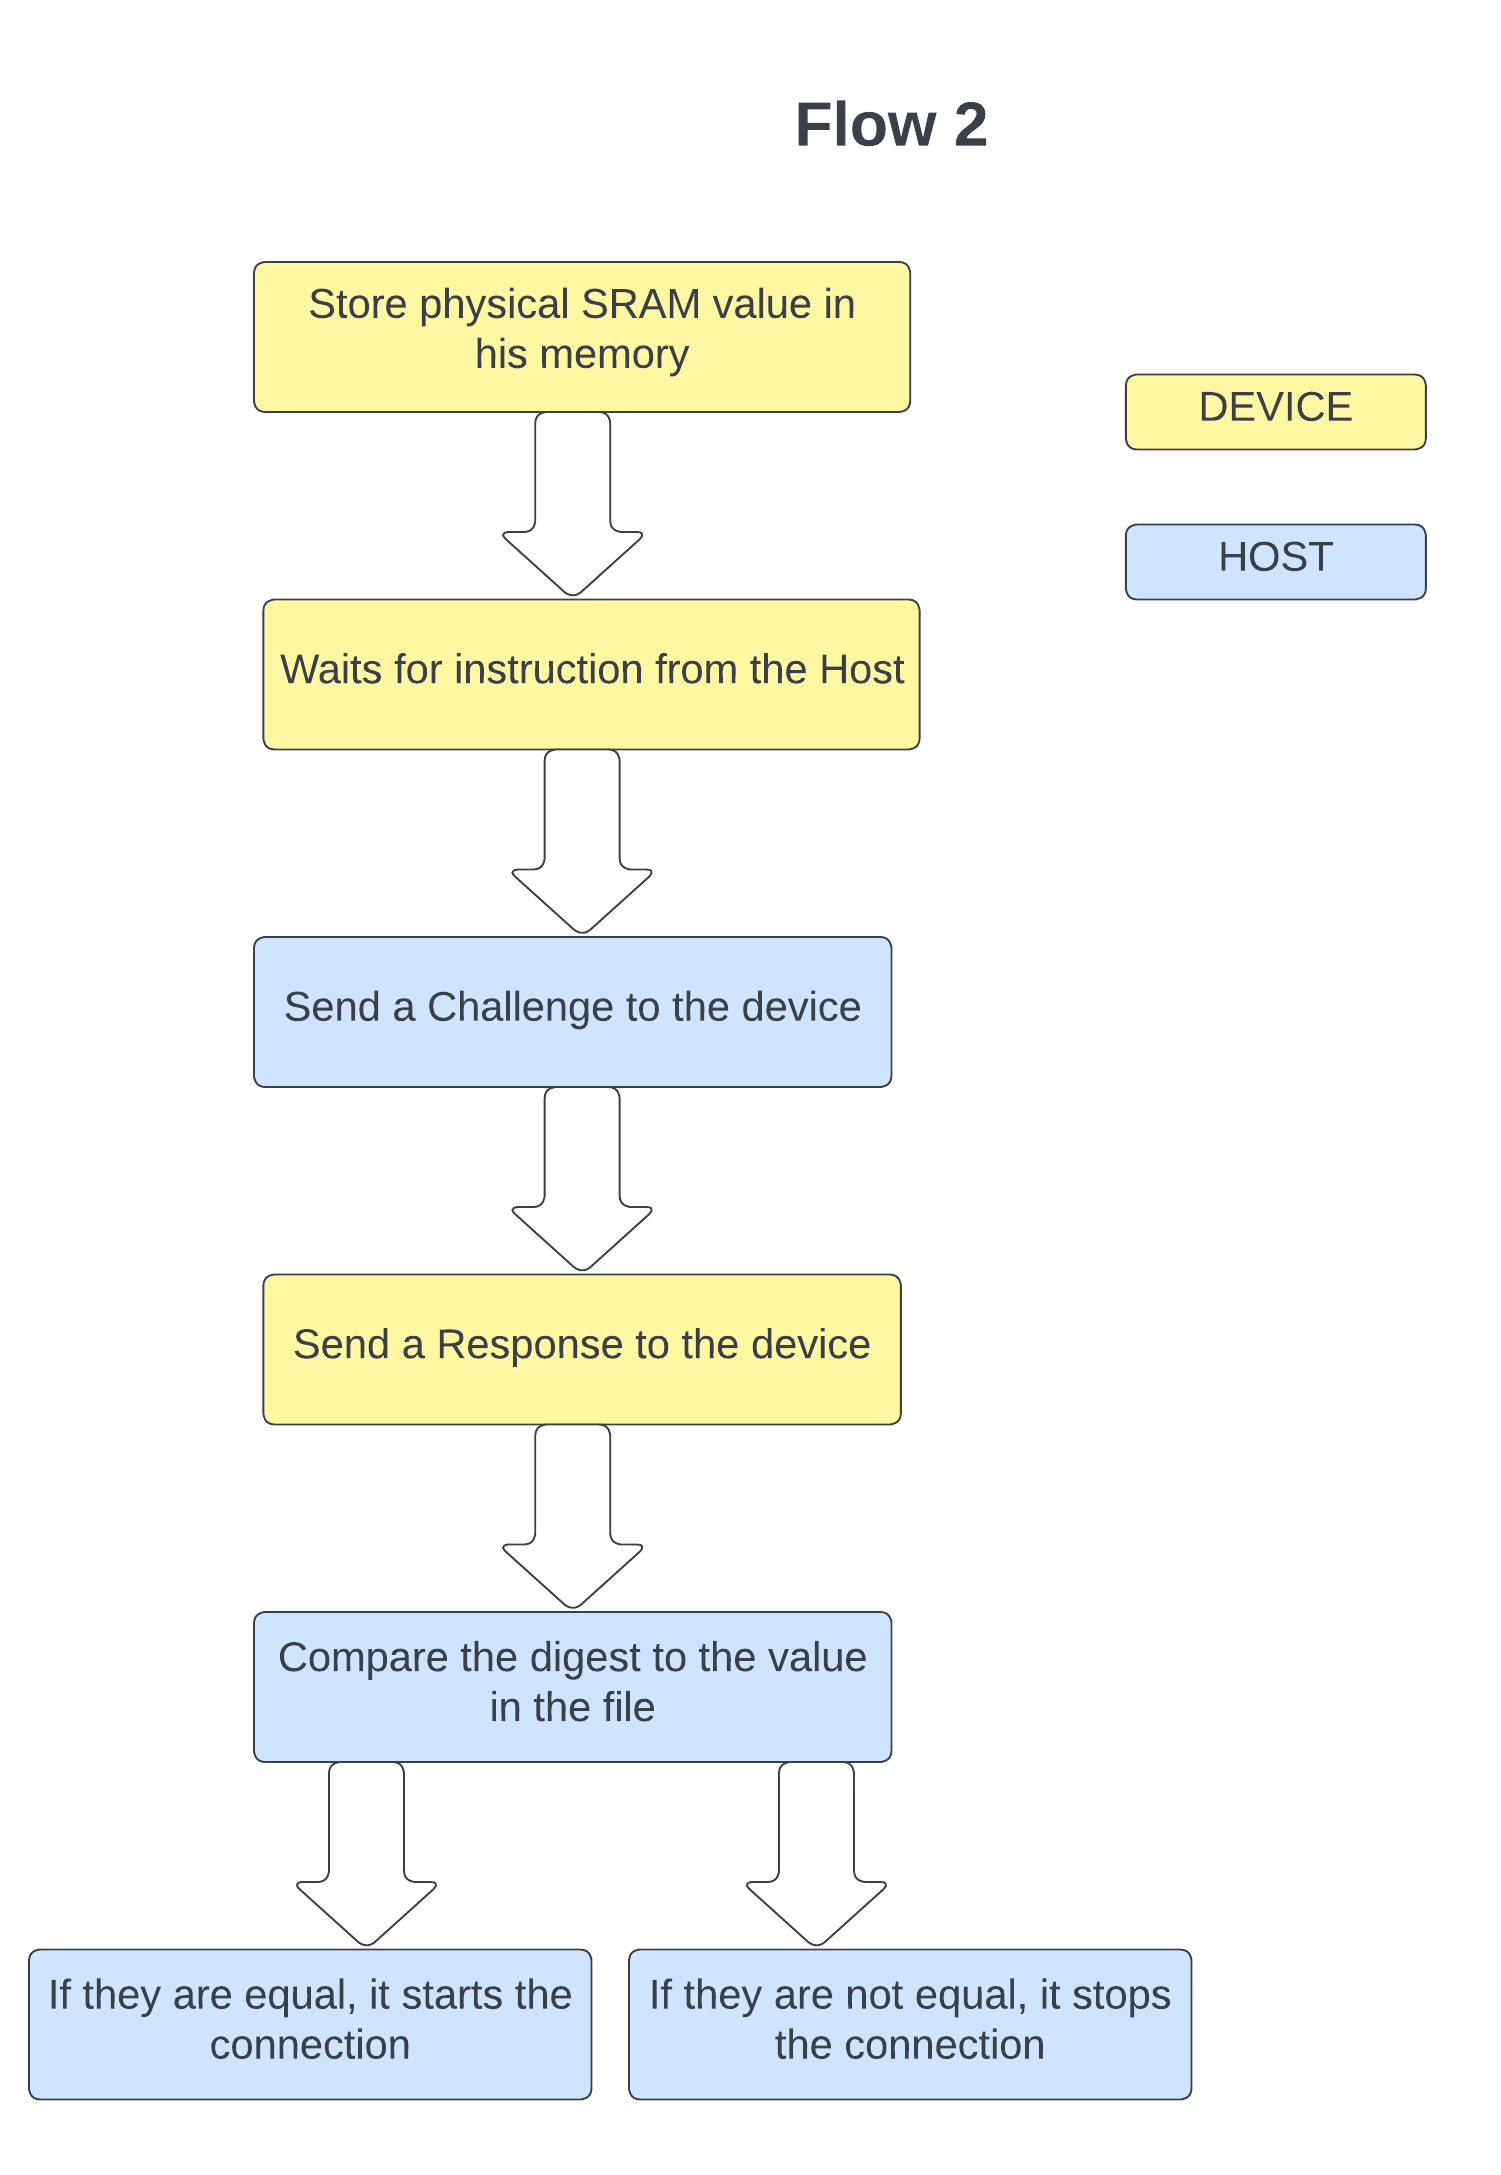
\includegraphics[width=5cm]{images/flow_2.png}
  \caption{Flow 1 and Flow 2}
  \label{fig:sub2}
\end{figure}

\section {Device side} 
On the device side both of the flows have a common important operation that has to be done. This operation consists in taking the values present in the SRAM when this one is switched on and storing them in a secure place. Obviously this operation is the first operation that has always been done by the device as soon as it is switched on.

Secondly, if this is the first time that it communicates with this particular host it waits until the host asks it for all the value that it has just taken from the SRAM in order to implement the challenge-response authentication for the next time.

On the other hand, it waits until the host sends to it a particular challenge, this challenge will be the index of a determined response, so the device takes the response and sends them to the host.
After that the device is authenticated and the can starts to communicate.



\section {Host side} 
On the host side the type of work is a little bit different from the device side.
When the connection is instantiated with the device for the first time it asks the device all the values needed to implement the challenge-response authentication; the Host is going to store the hash values of these datas in a file.

During all the next connections with the device, the Host sends a particular challenge to the device and waits for the respective response.
After it receives it, It is going to evaluate the digest of this value, it gives it in input to the hash function and it compares it with the value that it has inside the file.

If the two digests are the same it means that the device is the correct one and so the connection can start; otherwise the host stops the connection.



%In this chapter you should provide a general overview of the project, explaining what you have implemented staying at a high-level of abstraction, without going too much into the details. Leave details for the implementation chapter. This chapter can be organized in sections, such as goal of the project, issues to be solved, solution overview, etc.\\It is very important to add images, schemes, graphs to explain the original problem and your solution. Pictures are extremely useful to understand complex ideas that might need an entire page to be explained.\\Use multiple sections to explain the starting point of your project, the last section is going to be the high-level view of your solution...so take the reader in a short `journey` to showcase your work.
